\documentclass{article}
\usepackage{amsmath}
\usepackage{amssymb}
\usepackage{tikz}
\usetikzlibrary{calc}

\begin{document}

\title{Analysis of problem URI 1636 --- Cyclic Antimonotonic Permutations}
\date{}
\author{Tiago Royer}
\maketitle

The problem asks us to generate a permutation of $\{1, \dots, n\}$
that is both antimonotonic and cyclic.
To analyse the problem, we will use the divide-and-conquer approach.

First, let's take care of cyclicity.
If we have two disjoint cycles in a permutation
(like in figure~\ref{fig1}),
we can choose one edge from one cycle
and one edge from the other cycle and cross them over.

\begin{figure}[h]
    \centering
    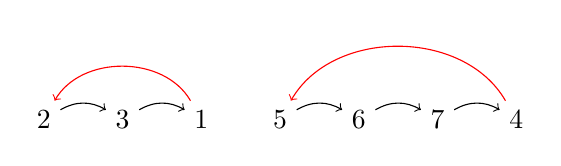
\begin{tikzpicture}
        \node (a) at (0, 0) {$2$};
        \node (b) at (1, 0) {$3$};
        \node (c) at (2, 0) {$1$};

        \node (d) at (3, 0) {$5$};
        \node (e) at (4, 0) {$6$};
        \node (f) at (5, 0) {$7$};
        \node (g) at (6, 0) {$4$};

        \draw[bend left=30, ->] (a) to (b);
        \draw[bend left=30, ->] (b) to (c);
        \draw[red, out=-60, in=-120, relative, ->] (c) to (a);

        \draw[bend left=30, ->] (d) to (e);
        \draw[bend left=30, ->] (e) to (f);
        \draw[bend left=30, ->] (f) to (g);
        \draw[red, out=-60, in=-120, relative, ->] (g) to (d);
    \end{tikzpicture}
    \caption{Two disjoint cycles in a permutation.}
    \label{fig1}
\end{figure}

In the example, we crossed the red edges.
The node labeled $1$ must now point to what the other node was pointing,
namely, the value $4$.
And the node labeled $4$ must now point to what the first node was pointing,
namely, the value $1$.
The result is depicted in figure~\ref{fig2}.

\begin{figure}[h]
    \centering
    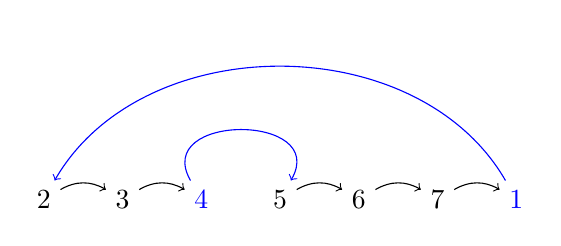
\begin{tikzpicture}
        \node (a) at (0, 0) {$2$};
        \node (b) at (1, 0) {$3$};
        \node[blue] (c) at (2, 0) {$4$};

        \node (d) at (3, 0) {$5$};
        \node (e) at (4, 0) {$6$};
        \node (f) at (5, 0) {$7$};
        \node[blue] (g) at (6, 0) {$1$};

        \draw[bend left=30, ->] (a) to (b);
        \draw[bend left=30, ->] (b) to (c);
        \draw[blue, out=120, in=60, relative, looseness=2, ->] (c) to (d);

        \draw[bend left=30, ->] (d) to (e);
        \draw[bend left=30, ->] (e) to (f);
        \draw[bend left=30, ->] (f) to (g);
        \draw[blue, out=-60, in=-120, relative, ->] (g) to (a);
    \end{tikzpicture}
    \caption{The two cycles, joined together.}
    \label{fig2}
\end{figure}

We will call this procedure a \emph{surgery}.
Note that the surgery simply swapped the two values;
so, a surgery is an $O(1)$ operation.
Also, observe that the surgery could be done using
any pair of edges,
by swapping the base node of each edge.
Therefore, besides being cheap,
a surgery is a very flexible operation.

Now, we will study antimonotonicity.
If $p_1, p_2, p_3$ is an antimonotonic sequence
with $p_2$ being the minimum,
then, when adding an extra $p_4$ value in the sequence,
$p_3$ automatically must be a maximum point:
Either $p_3$ is greater than both $p_2$ and $p_4$,
or $p_3$ is smaller than both $p_2$ and $p_4$.
The latter cannot happen,
since $p_2$ is a minimum point and hence smaller than $p_3$.
Thus, $p_3 > p_4$.
A similar argument can be repeated to show that
an hypothetical $p_5$ would need to be \emph{larger} than $p_4$,
and $p_6$ \emph{smaller} than $p_5$,
and $p_7$ \emph{larger}, and so on.

For the same reason, if $p_2$ starts as a local maximum,
the remaining sequence also alternates between high and low values.

Now, observe the following:
if we have two cycles side-by-side,
as in figure~\ref{fig1},
every value in the left cycle is smaller than every value in the right cycle.
Thus, any surgery will \emph{increase} the chosen node's value in the left cycle
(since that value will be swapped for a value in the right cycle,
which is necessarily greater),
and \emph{decrease} the corresponding value in the right cycle
(since that value wil be swapped for a value in the left cycle,
which is necessarily smaller).

Therefore, if we choose a maximum point in the left cycle
and a minimum point in the right cycle (figure~\ref{fig3}),
we will keep the antimonotonicity of the resulting sequence,
since the maximum point will be made even larger
and the minimum point will be made even smaller (figure~\ref{fig4}).

\begin{figure}[h]
    \centering
    \begin{tikzpicture}
        \draw (0, 0.5) -- (1, 1) -- (2, 0);
        \draw (3, 2.5) -- (4, 1.5) -- (5, 3) -- (6, 2);
        \draw[red, out=90, in=105, looseness=2, dashed] (1, 1) to (6, 2);
    \end{tikzpicture}
    \caption[Antimonotonic sequence before the surgery]{
        Antimonotonic sequence before the surgery.
        In red, the chosen two points for swapping.
    }
    \label{fig3}
\end{figure}

\begin{figure}[h]
    \centering
    \begin{tikzpicture}
        \draw (0, 0.5) -- (1, 2) -- (2, 0);
        \draw (3, 2.5) -- (4, 1.5) -- (5, 3) -- (6, 1);
        \draw[green, dashed] (0, 0.5) -- (1, 1) -- (2, 0);
        \draw[green, dashed] (5, 3) -- (6, 2);
        \draw[dashed, blue] (2, 0) -- (3, 2.5);
    \end{tikzpicture}
    \caption[Antimonotonic sequence after the surgery.]{
        Antimonotonic sequence after the surgery.
        In green, where the line passed before the surgery.
    }
    \label{fig4}
\end{figure}

In the example,
the first point of the right cycle was a maximum point
and the last point of the left cycle was a minimum point,
so, when pasted together,
they mantained the antimonotonicity.
Therefore,
if we find an efficient way to generate smaller cyclic antimonotonic permutations
satisfying,
at our choice,
the property of starting with a maximum point or a minimum point,
we can combine them together in a larger cyclic antimonotonic permutation.
This calls for a recursive algorithm.

But there is a simpler alternative.
Note that this argument holds for arbitrarily-sized antimonotonic permutations.
In particular, given a permutation
\begin{equation*}
    p_1, p_2, \dots, p_{n-1}, p_n
\end{equation*}
whose last value ($p_n$) is a minimum point,
we can paste the permutation $2, 1$ at the end,
leaving
\begin{equation*}
    p_1, p_2, \dots, p_{n-1}, p_n, n+2, n+1.
\end{equation*}
Note that this permutation is antimonotonic,
so if we can perform a surgery to join the two cycles,
we have a $n+2$-sized cyclic antimonotonic permutation.
But this is simple, since $n+1$ is our desired minimum point in the right,
and $p_{n-1}$ is our desired maximum point in the left.
($p_{n-1}$ must be larger than $p_n$ because $p_n$ is a minimum point,
so, as the sequence is antimonotonic, $p_{n-1}$ is a maximum point.)
After the surgery, we are left with the permutation
\begin{equation*}
    p_1, p_2, \dots, n+1, p_n, n+2, p_{n-1},
\end{equation*}
which is cyclic antimonotonic.

Therefore, if we can find a $3$-sized cyclic antimonotonic permutation,
we can generate a $n$-sized cyclic antimonotonic permutation
for any odd $n$,
and from a $2$-sized one,
we solve the problem for even $n$.

For the $2$-sized case we can pick the cycle $2, 1$ itself,
and the $3$-sized we chose $2, 3, 1$.

This alone is enough to implement an $O(n)$-time and space algorithm.
But we can make this algorithm use only $O(1)$ space.
Let's look at the first sequences generated by this algorithm:
\begin{align*}
    3:& 2, 3, 1 \\
    5:& 2, 4, 1, 5, 3 \\
    7:& 2, 4, 1, 6, 3, 7, 5 \\
    9:& 2, 4, 1, 6, 3, 8, 5, 9, 7 \\
    4:& 3, 1, 4, 2 \\
    6:& 3, 1, 5, 2, 6, 4 \\
    8:& 3, 1, 5, 2, 7, 4, 8, 6 \\
    10:& 3, 1, 5, 2, 7, 4, 9, 6, 10, 8 \\
\end{align*}

Notice that, if we look only at numbers in odd possitions
(or in even positions),
their values seems to almost always increase by two.
That is, for almost all indexes $i$,
\begin{equation*}
    p_{i+2} = p_i + 2.
\end{equation*}
By studying the larger cases,
we perceive that this relation only fail in the endpoints;
So, if we hardcode the first few values of each sequence
for both the even and odd cases,
we can construct the remainder of the sequence
storing only the last two used values,
thus yielding our $O(1)$-space algorithm.

We just need to deal with the end of the sequence.
Note that, both in even and odd case,
the last two numbers are $n$ and $n-2$, respectively;
this solves our problem.

But we may go further in the analysis.
We can use the linear relation above to show a simple formula,
in the form $ai+b$,
for every value in the sequence.
For $n$ odd, we have
\begin{equation*}
    p_i = \begin{cases}
        2, &\text{if $i = 1$} \\
        n, &\text{if $i = n-1$} \\
        i - 2, &\text{if $i$ is odd, but $i \neq 1$} \\
        i + 2, &\text{otherwise ($i$ even and $i \neq n-1$)} \\
    \end{cases}
\end{equation*}
(Observe that the rule for $i$ odd matches the case $i = n-1$.)

Similarly, for $n$ even, we have
\begin{equation*}
    p_i = \begin{cases}
        1, &\text{if $i = 2$} \\
        n, &\text{if $i = n-1$} \\
        i + 2, &\text{if $i$ is odd, but $i \neq n-1$} \\
        i - 2, &\text{otherwise ($i$ even and $i \neq 2$)} \\
    \end{cases}
\end{equation*}

Using these formulas, one can show by induction that
the modification in the algorithm (to make it $O(1)$) is correct.

In fact, one may show directly from these formulas
that the generated sequence is both cyclic and antimonotonic.
This proof shows one interesting property of the cycle:
for $n$ odd, the even $i$ will point to the index $i+2$ in the permutation.
Thus, the even indexes form a ``chain''
that carries up to the end of the sequence.
And the odd $i$ point to $i-2$,
thus forming a chain that carries us to the sequence.
Similarly, for even $n$, the odd $i$ ``moves up'' and even $i$ ``moves down''.
And the endpoints connects the two chains.

\end{document}
